\section{Auswertung}
\label{sec:Auswertung}

\begin{table}
  \centering
  \caption{Messung der Biegung des eckigen Stabs bei einseitiger Einspannung}
  \label{tab:ecks}
  \sisetup{table-format=2.1}
  \begin{tabular}{S[table-format=4.0] S[table-Sformat=4.0]}
    \toprule
    {$x \mathbin{/} \si{\milli\meter}$} & {$D(x) \mathbin{/} \si{\milli\meter}$}
  \end{tabular}
\end{table}

\begin{figure}
  \centering
  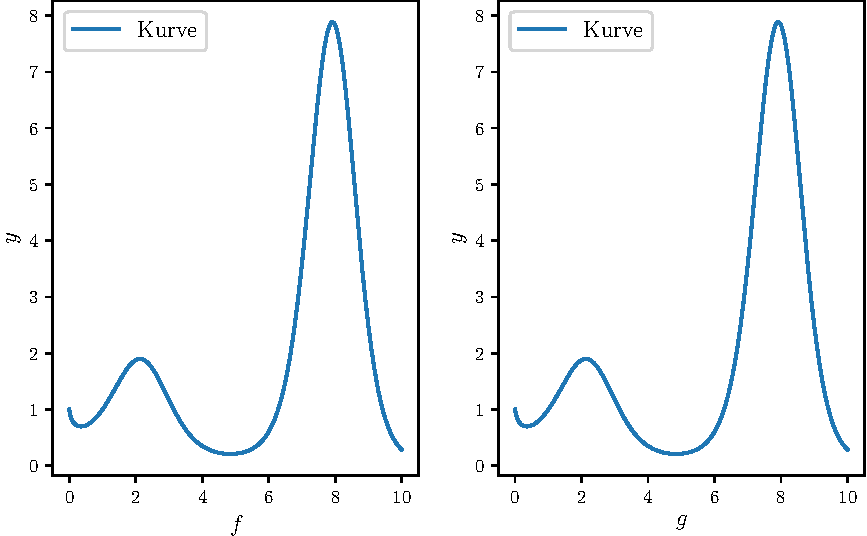
\includegraphics{plot.pdf}
  \caption{Plot.}
  \label{fig:plot}
\end{figure}


Siehe \autoref{fig:plot}!
